% !TEX root = ../Main.tex

\subsection{Lattice Geometry}
In order to set up the simulation environment the basic geometry of system must be defined. Using generating vectors as well as unitcells the structure and holes of the graphene sheet will be defined within this geometry.
\subsubsection{Bravais Lattice \& Generating Vectors}\label{BLGV}
At first we want to specify a Bravais lattice for the graphene-layer. The Bravais lattice is a lattice that is invariant under translation which means that the lattice doesn't change when you translate it with the vector
\begin{equation}
 \mathbf{T}=n\mathbf{a_{1}}+m\mathbf{a_{2}}\ \ \ \mathbf{a_{1}},\mathbf{a_{2}} \in \mathbb{R}^{2}
\end{equation}
Where $n,m \in \mathbb{Z}$ and $\mathbf{a_{1}}$, $\mathbf{a_{2}}$ are the generating vectors for the space lattice. Moreover, all the points in the lattice are given by
\begin{equation}
 \mathbf{R}=(nd,md)
\end{equation}
where $d$ is the spacing between the lattice points and $n,m$ can be both positive and negative integers. \\
As we are working with graphene which is carbon atoms arranged in a hexagonal structure, we want to choose a hexagonal Bravais lattice and define our generating vectors accordingly. Both generating vectors start at the center of a hexagon. This gives the generating vectors $\mathbf{a_{1}}=(d,0)$ \& $\mathbf{a_{2}}=\left(-\dfrac{d}{2},\dfrac{\sqrt{3}d}{2}\right)$. In \cref{hexagon} a drawing of the lattice with its generating vectors is shown.\\
As the carbon-carbon bondlength in graphene is \SI{1.42}{\angstrom}, the distance between the lattice points  in the Bravais lattice is $d=\SI{2.4612}{\angstrom}$. This gives the numerical form of the analytical derived expression for the generating vectors  $\mathbf{a_{1}}$ \& $\mathbf{a_{2}}$. \\
$\mathbf{a_{1}}=(\SI{2.4612}{\angstrom},0)$ \& $\mathbf{a_{2}}=\left(-\SI{1.2306}{\angstrom},\SI{2.1315}{\angstrom}\right)$. \\These are the vectors that will be employed during simulation.
\begin{figure}
 \centering
 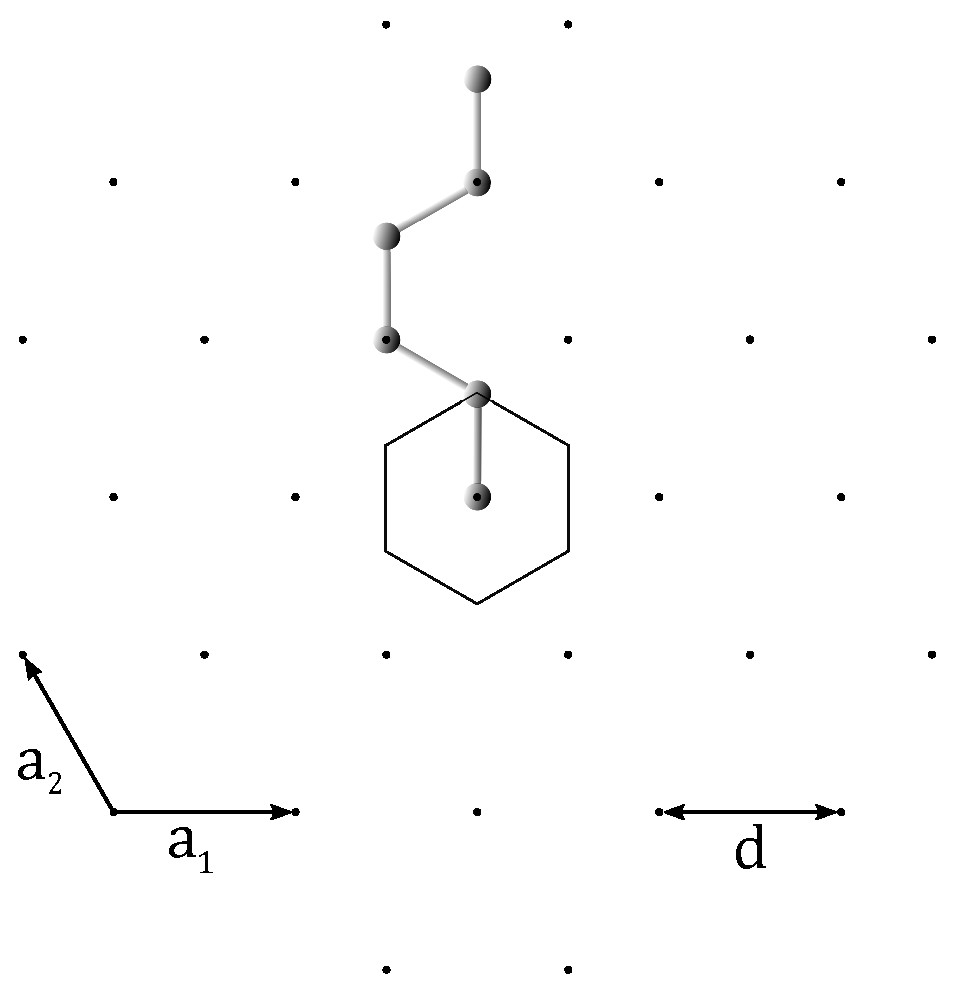
\includegraphics[width=0.5\textwidth]{Figures/hexagon2.eps}
 \caption{Hexagonal Bravais lattice structure with generating vectors $\mathbf{a_{1}}$ \& $\mathbf{a_{2}}$. The Hexagon in the middle with the solid lines is unit cell and the shaded elements are the carbon atoms placed in the lattice.}
 \label{hexagon}
\end{figure}
